
%Page ??
\newpage
\changefontsizes{16pt}
\centerline{\textbf{CHƯƠNG III: VÍ DỤ MINH HỌA}}
\centerline{\textbf{DỰ BÁO THỜI TIẾT}}

\vspace{1cm}
\changefontsizes{15pt}
\setlength{\parindent}{0cm}
\textbf{Chuẩn bị}

\vspace{0.25cm}
\changefontsizes{14pt}
\setlength{\parindent}{0cm}
\textbf{Môi trường}

\vspace{0.5cm}
\changefontsizes{13pt}
- Sử dụng python 3.8\\
- Trình soạn thảo Jupyter notebook\\
- Package: tensorflow, matplotlib, numpy, os, pandas


\vspace{0.75cm}
\changefontsizes{14pt}
\setlength{\parindent}{0cm}
\textbf{Dữ liệu}


\vspace{0.5cm}
\changefontsizes{13pt}
- Tập dữ \href{https://www.bgc-jena.mpg.de/wetter/}{\textcolor{blue}{liệu thời tiết}} được cung cấp bởi  \href{https://www.bgc-jena.mpg.de/index.php/Main/HomePage}{\textcolor{blue}{Max Planck Institute for Biogeochemistry}}.

\bigskip
- Tập dữ liệu này chứa 14 loại đặc điểm khác nhau của thời tiết như: nhiệt độ (temperature), áp suất không khí (atmospheric), độ ẩm (humidity),... Các giá trị này sẽ được ghi lại cứ mỗi 10 phút, bắt đầu từ năm 2009 đến 2016. Phần dữ liệu này đã được chỉnh sửa lại bởi François Chollet.

\vspace{0.75cm}
\changefontsizes{15pt}
\setlength{\parindent}{0cm}
\textbf{Mục tiêu}


\vspace{0.5cm}
\changefontsizes{13pt}
Với dữ liệu đã có, sử dụng mô hình RNN để dự đoán nhiệt độ của 6 giờ kế tiếp qua hai trường hợp: đơn biến (univariate) và đa biến (multivariate)


\vspace{0.75cm}
\changefontsizes{15pt}
\setlength{\parindent}{0cm}
\textbf{Code}


\vspace{0.25cm}
\changefontsizes{14pt}
\setlength{\parindent}{0cm}
\textbf{Khai báo các package cần thiết}

\begin{lstlisting}[language=Python]
import tensorflow as tf

import matplotlib as mpl
import matplotlib.pyplot as plt
import numpy as np
import os
import pandas as pd

mpl.rcParams['figure.figsize'] = (8, 6)
mpl.rcParams['axes.grid'] = False
\end{lstlisting}


\vspace{0.25cm}
\changefontsizes{14pt}
\setlength{\parindent}{0cm}
\textbf{Tải dữ liệu}


\begin{lstlisting}[language=Python]
zip_path = tf.keras.utils.get_file(
origin='https://storage.googleapis.com/tensorflow/tf-keras-datasets/jena_climate_2009_2016.csv.zip',
fname='jena_climate_2009_2016.csv.zip',
extract=True)
csv_path, _ = os.path.splitext(zip_path)
df = pd.read_csv(csv_path)
\end{lstlisting}


\vspace{0.25cm}
\changefontsizes{13pt}
\setlength{\parindent}{0cm}
\textbf{Xem thử bảng dữ liệu}

\begin{lstlisting}[language=Python]
df.head()
\end{lstlisting}


\vspace{0.25cm}
\changefontsizes{13pt}
\setlength{\parindent}{0cm}
Nếu kết quả in ra có dạng như thế này, thì xem như việc tải dữ liệu thành công.

\vspace{-0.5cm}
\begin{center}
	\begin{figure}[h]
		\begin{center}
			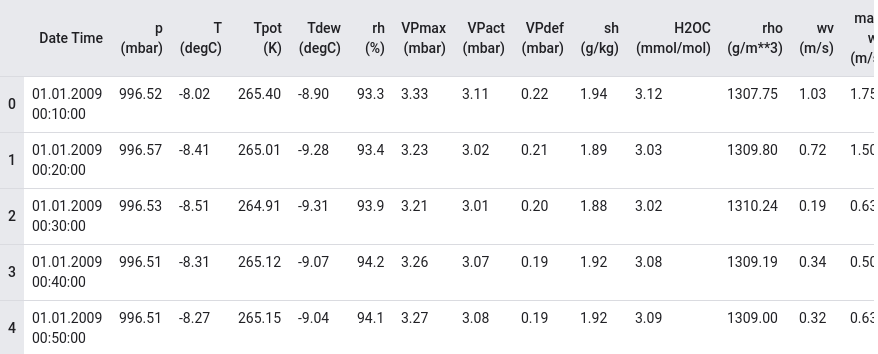
\includegraphics[scale=0.52]{./images/tables.png}
		\end{center}
	\end{figure}
\end{center}

Từ bảng trên ta thấy, cứ mỗi giờ thì có 6 quan sát được ghi lại. Vậy nên mỗi ngày sẽ có 144 (6 $\times$ 24) quan sát.

\smallskip
Với mục tiêu dự đoán nhiệt độ của 6 giờ kế tiếp. Ta thử chọn ra 5 ngày quan sát trước đó. Tức là ta sẽ lấy 720 (5 $\times$ 144) quan sát. Tương ứng ta sẽ có 2 tham số `history\_size` biểu diễn cho số quan sát trước đó và `target\_size` là số quan sát cần dự đoán. 


\vspace{0.25cm}
\changefontsizes{13pt}
\setlength{\parindent}{0cm}
Ta dùng 300,000 hàng đầu tiên của tập dữ liệu để làm tập dữ liệu huấn luyện, phần còn lại sẽ làm dữ liệu kiểm thử.

\begin{lstlisting}[language=Python]
TRAIN_SPLIT = 300000
tf.random.set_seed(13) #Setting seed to ensure reproducibility.
\end{lstlisting}


\vspace{0.25cm}
\changefontsizes{14pt}
\setlength{\parindent}{0cm}
\textbf{Dự đoán với đơn biến}


\vspace{0.25cm}
\changefontsizes{13pt}
Với trường hợp này ta sẽ chỉ dùng một giá trị duy nhất là nhiệt độ, để dự đoán nhiệt độ trong tương lai.

\begin{lstlisting}[language=Python]
uni_data = df['T (degC)']
uni_data.index = df['Date Time']
uni_data.head()
\end{lstlisting}

Xem thử dữ liệu

\begin{lstlisting}[language=Python]
uni_data.plot(subplots=True)
uni_data = uni_data.values
\end{lstlisting}


\vspace{-1cm}
\begin{center}
	\begin{figure}[htp]
		\begin{center}
			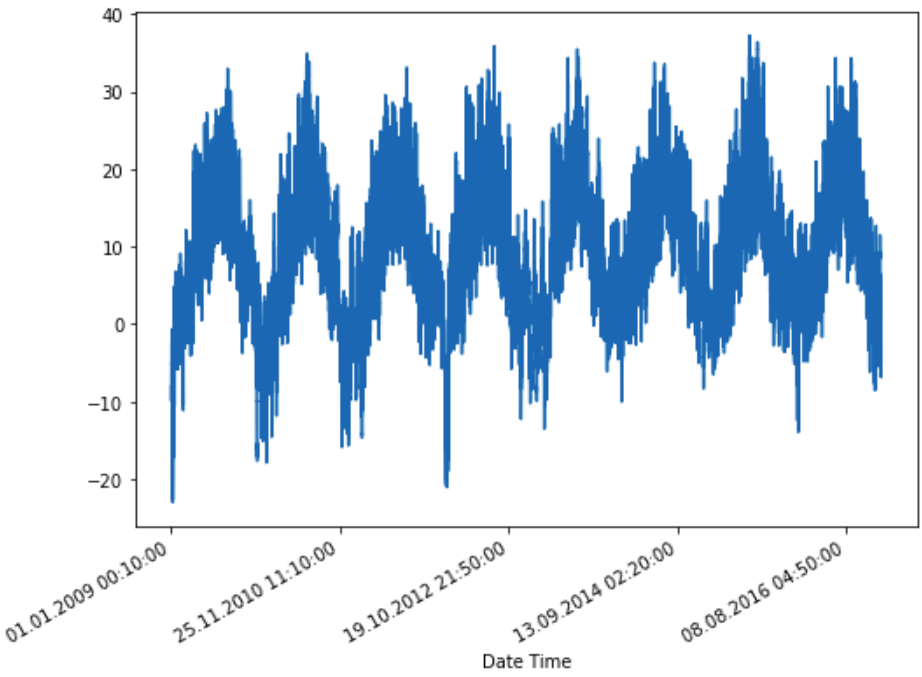
\includegraphics[scale=0.3]{./images/1.png}
		\end{center}
	\end{figure}
\end{center}

Để cho mô hình hoạt động hiệu quả, chính xác hơn, ta cần chuẩn hóa dữ liệu trước khi cho đi huấn luyện.


\begin{lstlisting}[language=Python]
uni_train_mean = uni_data[:TRAIN_SPLIT].mean()
uni_train_std = uni_data[:TRAIN_SPLIT].std()
uni_data = (uni_data-uni_train_mean)/uni_train_std
\end{lstlisting}


\vspace{0.25cm}
\changefontsizes{13pt}
\setlength{\parindent}{0cm}
\textbf{Chế biến dữ liệu lại thành tập dữ liệu huấn luyện}


\begin{lstlisting}[language=Python]
def univariate_data(dataset, start_index, end_index, history_size, target_size):
	data = []
	labels = []
	
	start_index = start_index + history_size
	if end_index is None:
		end_index = len(dataset) - target_size
	
	for i in range(start_index, end_index):
		indices = range(i-history_size, i)
		# Reshape data from (history_size,) to (history_size, 1)
		data.append(np.reshape(dataset[indices], (history_size, 1)))
		labels.append(dataset[i+target_size])
	return np.array(data), np.array(labels)
	

univariate_past_history = 20
univariate_future_target = 0

x_train_uni, y_train_uni = univariate_data(uni_data, 0, TRAIN_SPLIT, univariate_past_history, univariate_future_target)
x_val_uni, y_val_uni = univariate_data(uni_data, TRAIN_SPLIT, None,
univariate_past_history,
univariate_future_target)
\end{lstlisting}


Vậy là ta đã chuẩn bị xong dữ liệu, hãy xem thử nó trông như thế nào.


\begin{lstlisting}[language=Python]
def create_time_steps(length):
	return list(range(-length, 0))

def show_plot(plot_data, delta, title):
	labels = ['History', 'True Future', 'Model Prediction']
	marker = ['.-', 'rx', 'go']
	time_steps = create_time_steps(plot_data[0].shape[0])
	if delta:
		future = delta
	else:
		future = 0
	
	plt.title(title)
	for i, x in enumerate(plot_data):
		if i:
			plt.plot(future, plot_data[i], marker[i], markersize=10,
			label=labels[i])
		else:
			plt.plot(time_steps, plot_data[i].flatten(), marker[i], label=labels[i])
	plt.legend()
	plt.xlim([time_steps[0], (future+5)*2])
	plt.xlabel('Time-Step')
	return plt

show_plot([x_train_uni[0], y_train_uni[0]], 0, 'Sample Example')
\end{lstlisting}



\vspace{-1cm}
\begin{center}
	\begin{figure}[htp]
		\begin{center}
			
\includegraphics[scale=0.3]{./images/2.png}
		\end{center}
	\end{figure}
\end{center}


\vspace{2cm}
\changefontsizes{13pt}
\setlength{\parindent}{0cm}
\textbf{Tiến hành huấn luyện}



\begin{lstlisting}[language=Python]
BATCH_SIZE = 256
BUFFER_SIZE = 10000

train_univariate = tf.data.Dataset.from_tensor_slices((x_train_uni, y_train_uni))
train_univariate = train_univariate.cache().shuffle(BUFFER_SIZE).batch(BATCH_SIZE).repeat()

val_univariate = tf.data.Dataset.from_tensor_slices((x_val_uni, y_val_uni))
val_univariate = val_univariate.batch(BATCH_SIZE).repeat()

simple_lstm_model = tf.keras.models.Sequential([
tf.keras.layers.LSTM(8, input_shape=x_train_uni.shape[-2:]),
tf.keras.layers.Dense(1)
])

simple_lstm_model.compile(optimizer='adam', loss='mae')

simple_lstm_model = tf.keras.models.Sequential([
tf.keras.layers.LSTM(8, input_shape=x_train_uni.shape[-2:]),
tf.keras.layers.Dense(1)
])

simple_lstm_model.compile(optimizer='adam', loss='mae')

EVALUATION_INTERVAL = 200
EPOCHS = 10

simple_lstm_model.fit(train_univariate, epochs=EPOCHS,
steps_per_epoch=EVALUATION_INTERVAL,
validation_data=val_univariate, validation_steps=50)
\end{lstlisting}



\vspace{0.25cm}
\changefontsizes{13pt}
\setlength{\parindent}{0cm}
\textbf{Thử một vài dự đoán}


\begin{lstlisting}[language=Python]
for x, y in val_univariate.take(3):
plot = show_plot([x[0].numpy(), y[0].numpy(),
simple_lstm_model.predict(x)[0]], 0, 'Simple LSTM model')
plot.show()
\end{lstlisting}





\vspace{-1cm}
\begin{center}
	\begin{figure}[htp]
		\begin{center}
			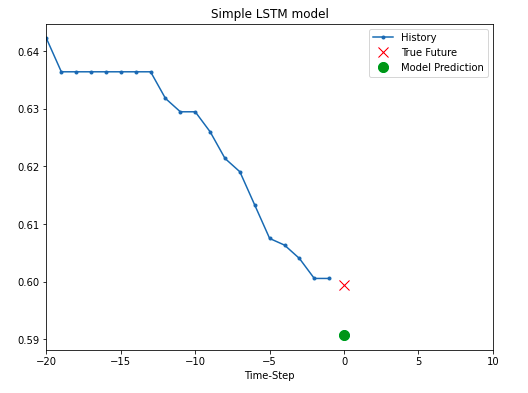
\includegraphics[scale=0.5]{./images/3.png}
		\end{center}
	\end{figure}
\end{center}




\vspace{-1cm}
\begin{center}
	\begin{figure}[htp]
		\begin{center}
			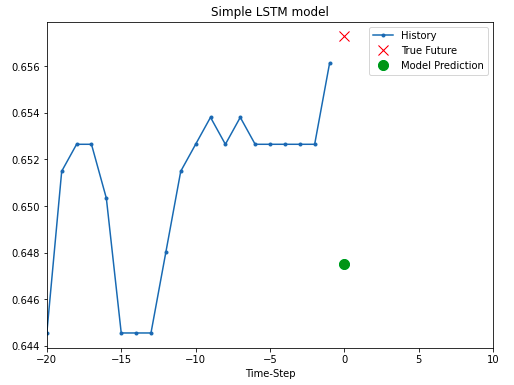
\includegraphics[scale=0.5]{./images/4.png}
		\end{center}
	\end{figure}
\end{center}




\vspace{-1cm}
\begin{center}
	\begin{figure}[htp]
		\begin{center}
			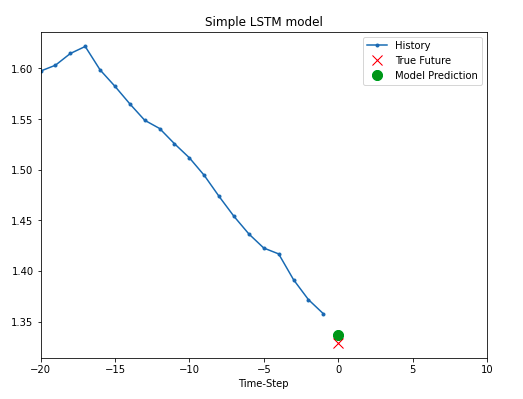
\includegraphics[scale=0.5]{./images/5.png}
		\end{center}
	\end{figure}
\end{center}



\vspace{5cm}
\changefontsizes{15pt}
\setlength{\parindent}{0cm}
\textbf{Dự đoán với đa biến}


\vspace{0.25cm}
\changefontsizes{14pt}
\setlength{\parindent}{0cm}
\textbf{Dự đoán một bước (one-step)}



\vspace{0.25cm}
\changefontsizes{13pt}
Với trường hợp này ta sẽ chỉ dùng 3 đặc trưng trong 14 đặc trưng trong tập dữ liệu, để dự đoán nhiệt độ trong tương lai.


\begin{lstlisting}[language=Python]
features_considered = ['p (mbar)', 'T (degC)', 'rho (g/m**3)']

features = df[features_considered]
features.index = df['Date Time']
\end{lstlisting}

Xem thử dữ liệu



\begin{lstlisting}[language=Python]
features.head()
features.plot(subplots=True)
\end{lstlisting}


\vspace{-0.75cm}
\begin{center}
	\begin{figure}[htp]
		\begin{center}
			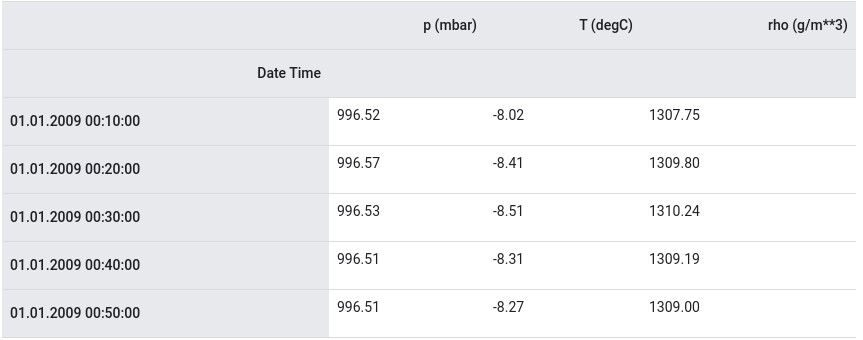
\includegraphics[scale=0.5]{./images/6.png}
		\end{center}
	\end{figure}
\end{center}



\vspace{-0.75cm}
\begin{center}
	\begin{figure}[htp]
		\begin{center}
			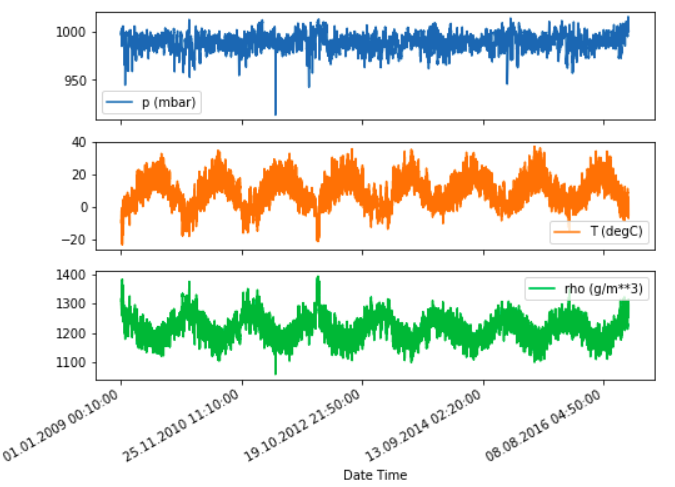
\includegraphics[scale=0.6]{./images/7.png}
		\end{center}
	\end{figure}
\end{center}


Tương tự như trên, ta cũng chuẩn hóa dữ liệu trước khi cho đi huấn luyện.



\begin{lstlisting}[language=Python]
dataset = features.values
data_mean = dataset[:TRAIN_SPLIT].mean(axis=0)
data_std = dataset[:TRAIN_SPLIT].std(axis=0)

dataset = (dataset-data_mean)/data_std
\end{lstlisting}




\vspace{0.25cm}
\changefontsizes{13pt}
\setlength{\parindent}{0cm}
\textbf{Chế biến dữ liệu lại thành tập dữ liệu huấn luyện}

\begin{lstlisting}[language=Python]
def multivariate_data(dataset, target, start_index, end_index, history_size,
	target_size, step, single_step=False):
	data = []
	labels = []
	
	start_index = start_index + history_size
	if end_index is None:
		end_index = len(dataset) - target_size
	
	for i in range(start_index, end_index):
		indices = range(i-history_size, i, step)
		data.append(dataset[indices])
	
	if single_step:
		labels.append(target[i+target_size])
	else:
		labels.append(target[i:i+target_size])
	
	return np.array(data), np.array(labels)
	
past_history = 720
future_target = 72
STEP = 6

x_train_single, y_train_single = multivariate_data(dataset, dataset[:, 1], 0,
TRAIN_SPLIT, past_history,
future_target, STEP,
single_step=True)
x_val_single, y_val_single = multivariate_data(dataset, dataset[:, 1],
TRAIN_SPLIT, None, past_history,
future_target, STEP,
single_step=True)
\end{lstlisting}


\vspace{0.5cm}
\changefontsizes{13pt}
\setlength{\parindent}{0cm}
\textbf{Tiến hành huấn luyện}


\begin{lstlisting}[language=Python]
train_data_single = tf.data.Dataset.from_tensor_slices((x_train_single, y_train_single))
train_data_single = train_data_single.cache().shuffle(BUFFER_SIZE).batch(BATCH_SIZE).repeat()

val_data_single = tf.data.Dataset.from_tensor_slices((x_val_single, y_val_single))
val_data_single = val_data_single.batch(BATCH_SIZE).repeat()

single_step_model = tf.keras.models.Sequential()
single_step_model.add(tf.keras.layers.LSTM(32,
input_shape=x_train_single.shape[-2:]))
single_step_model.add(tf.keras.layers.Dense(1))

single_step_model.compile(optimizer=tf.keras.optimizers.RMSprop(), loss='mae')

single_step_history = single_step_model.fit(train_data_single, epochs=EPOCHS,
steps_per_epoch=EVALUATION_INTERVAL, validation_data=val_data_single, validation_steps=50)
\end{lstlisting}

Xem quá biểu đồ biểu diễn độ lỗi

\begin{lstlisting}[language=Python]
def plot_train_history(history, title):
	loss = history.history['loss']
	val_loss = history.history['val_loss']
	
	epochs = range(len(loss))
	
	plt.figure()
	
	plt.plot(epochs, loss, 'b', label='Training loss')
	plt.plot(epochs, val_loss, 'r', label='Validation loss')
	plt.title(title)
	plt.legend()
	
	plt.show()

plot_train_history(single_step_history,
'Single Step Training and validation loss')
\end{lstlisting}


\vspace{-0.75cm}
\begin{center}
	\begin{figure}[htp]
		\begin{center}
			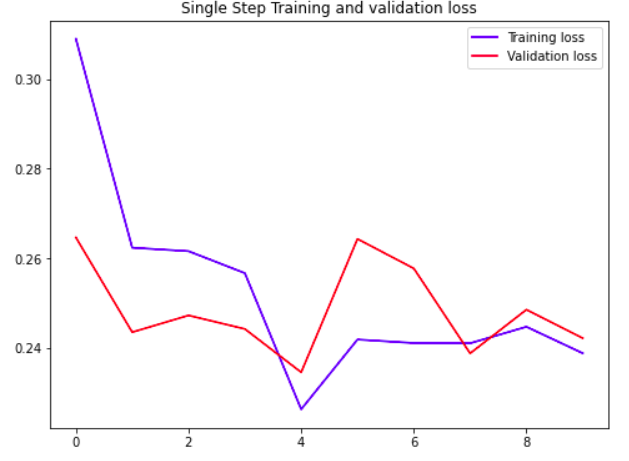
\includegraphics[scale=0.6]{./images/8.png}
		\end{center}
	\end{figure}
\end{center}



\vspace{0.25cm}
\changefontsizes{13pt}
\setlength{\parindent}{0cm}
\textbf{Thử một vài dự đoán}


\begin{lstlisting}[language=Python]
for x, y in val_data_single.take(3):
	plot = show_plot([x[0][:, 1].numpy(), y[0].numpy(),
	single_step_model.predict(x)[0]], 12,
	'Single Step Prediction')
plot.show()
\end{lstlisting}

\vspace{-1cm}
\begin{center}
	\begin{figure}[htp]
		\begin{center}
			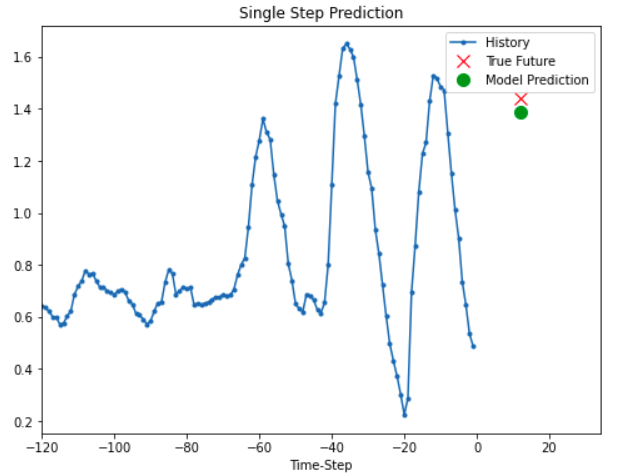
\includegraphics[scale=0.45]{./images/9.png}
		\end{center}
	\end{figure}
\end{center}


\vspace{-2cm}
\begin{center}
	\begin{figure}[htp]
		\begin{center}
			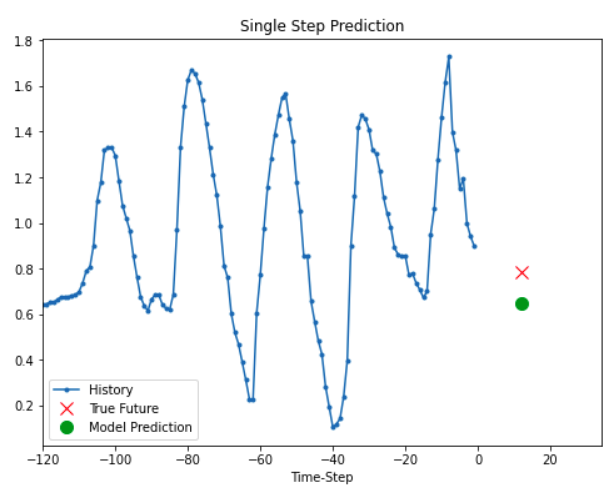
\includegraphics[scale=0.45]{./images/10.png}
		\end{center}
	\end{figure}
\end{center}


\begin{center}
	\begin{figure}[htp]
		\begin{center}
			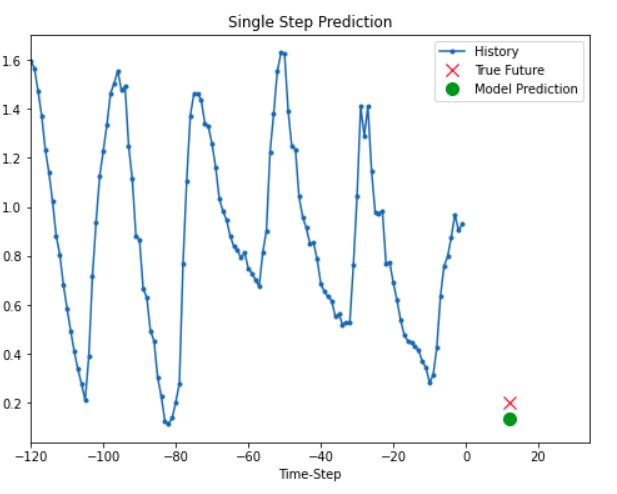
\includegraphics[scale=0.45]{./images/11.png}
		\end{center}
	\end{figure}
\end{center}


\vspace{5cm}
\changefontsizes{14pt}
\setlength{\parindent}{0cm}
\textbf{Dự đoán nhiều bước (Multi-step)}


Các bước bên dưới thực hiện tương tự như trên.

\begin{lstlisting}[language=Python]
future_target = 72
x_train_multi, y_train_multi = multivariate_data(dataset, dataset[:, 1], 0,
TRAIN_SPLIT, past_history,
future_target, STEP)
x_val_multi, y_val_multi = multivariate_data(dataset, dataset[:, 1],
TRAIN_SPLIT, None, past_history,
future_target, STEP)

train_data_multi = tf.data.Dataset.from_tensor_slices((x_train_multi, y_train_multi))
train_data_multi = train_data_multi.cache().shuffle(BUFFER_SIZE).batch(BATCH_SIZE).repeat()

val_data_multi = tf.data.Dataset.from_tensor_slices((x_val_multi, y_val_multi))
val_data_multi = val_data_multi.batch(BATCH_SIZE).repeat()

multi_step_model = tf.keras.models.Sequential()
multi_step_model.add(tf.keras.layers.LSTM(32,
return_sequences=True,
input_shape=x_train_multi.shape[-2:]))
multi_step_model.add(tf.keras.layers.LSTM(16, activation='relu'))
multi_step_model.add(tf.keras.layers.Dense(72))

multi_step_model.compile(optimizer=tf.keras.optimizers.RMSprop(clipvalue=1.0), loss='mae')

multi_step_history = multi_step_model.fit(train_data_multi, epochs=EPOCHS,
steps_per_epoch=EVALUATION_INTERVAL,
validation_data=val_data_multi,
validation_steps=50)
\end{lstlisting}

Xem vài kết quả dự đoán

\begin{lstlisting}[language=Python]
def multi_step_plot(history, true_future, prediction):
	plt.figure(figsize=(12, 6))
	num_in = create_time_steps(len(history))
	num_out = len(true_future)
	
	plt.plot(num_in, np.array(history[:, 1]), label='History')
	plt.plot(np.arange(num_out)/STEP, np.array(true_future), 'bo',
	label='True Future')
	if prediction.any():
		plt.plot(np.arange(num_out)/STEP, np.array(prediction), 'ro', label='Predicted Future')
	plt.legend(loc='upper left')
	plt.show()

for x, y in train_data_multi.take(1):
	multi_step_plot(x[0], y[0], np.array([0]))
\end{lstlisting}

\begin{center}
	\begin{figure}[htp]
		\begin{center}
			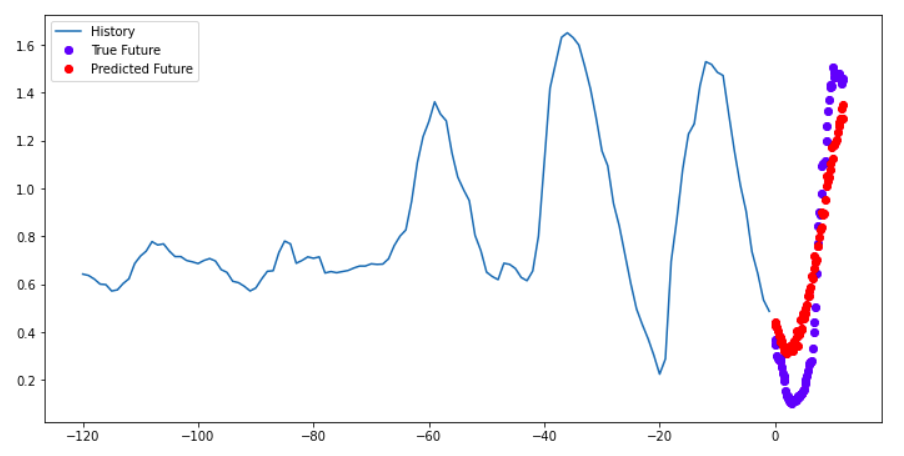
\includegraphics[scale=0.49]{./images/12.png}
		\end{center}
	\end{figure}
\end{center}


\begin{center}
	\begin{figure}[htp]
		\begin{center}
			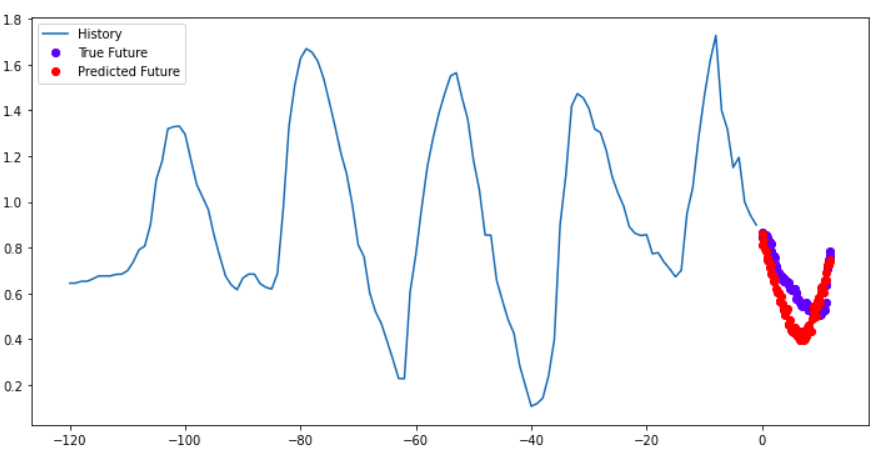
\includegraphics[scale=0.49]{./images/13.png}
		\end{center}
	\end{figure}
\end{center}


\begin{center}
	\begin{figure}[htp]
		\begin{center}
			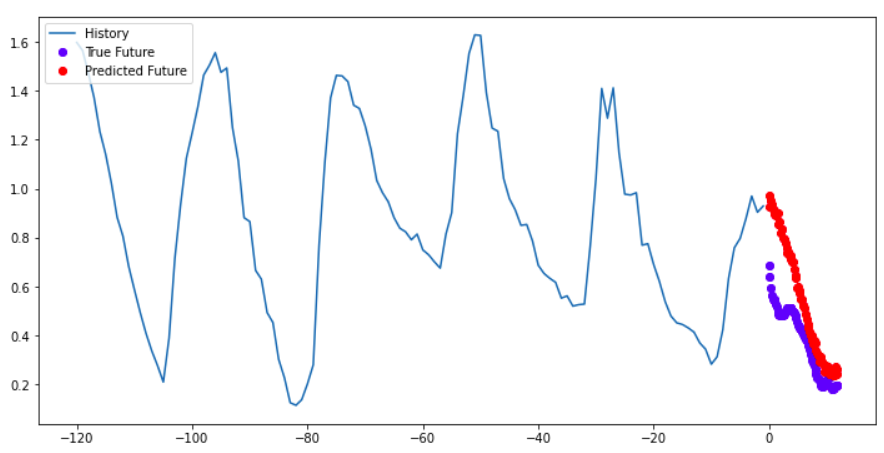
\includegraphics[scale=0.5]{./images/14.png}
		\end{center}
	\end{figure}
\end{center}

\newpage
.